\documentclass{resume}

\begin{document}

\fontfamily{ppl}\selectfont

\noindent
\begin{tabularx}{\linewidth}{@{}m{0.8\textwidth} m{0.2\textwidth}@{}}
{
    \textcolor{ceruleanblue}{\Large{Anna Fedorova}} \newline
    \textcolor{ceruleanblue}{\small\textbf{Software Engineer}} \newline
    \small{
        \clink{
            \href{mailto:anna.fedorova.se@gmail.com}{anna.fedorova.se@gmail.com} \newline
            {\fontdimen2\font=0.75ex +49 1520 7153706} 
        } \newline
        Stiftsbogen 70, 81375, Munich, Germany
    }
} & 
{
    %\hfill
    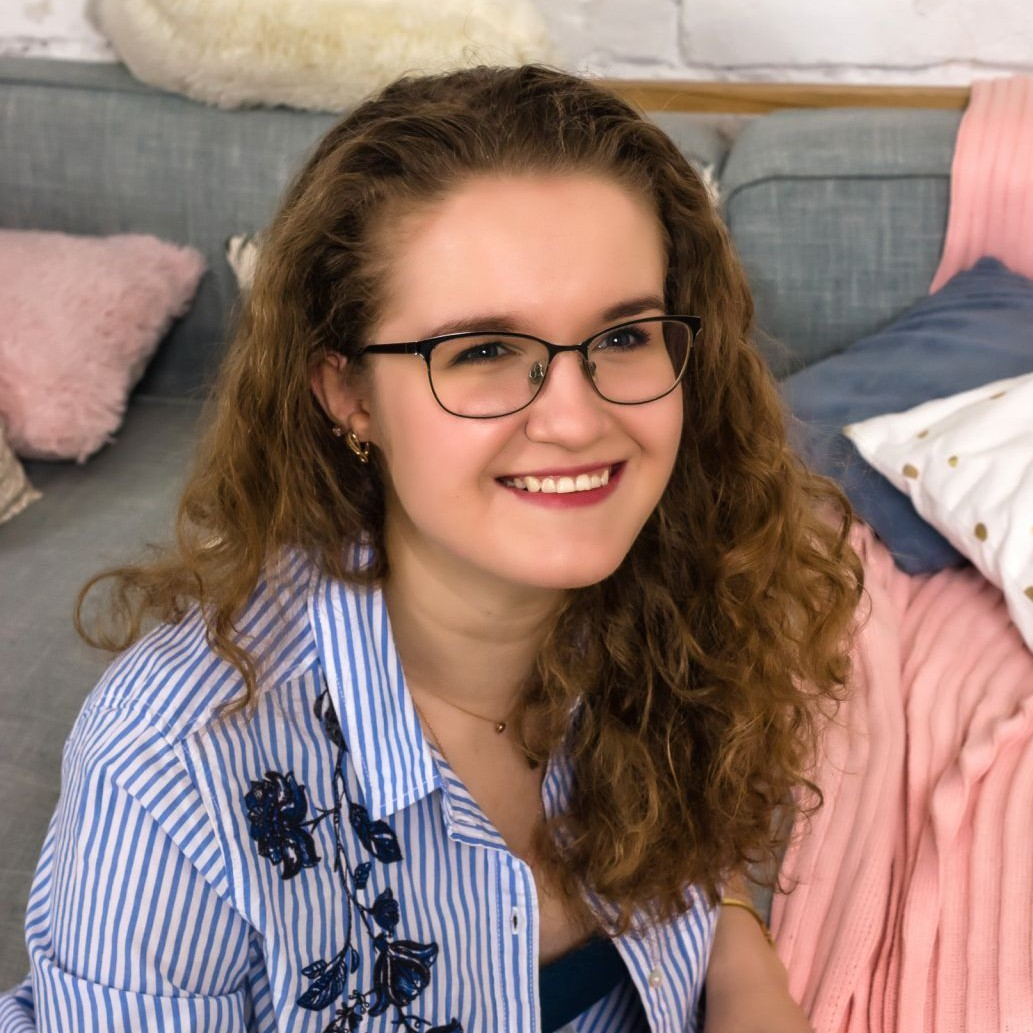
\includegraphics[width=2.8cm]{photo.jpg}
}
\end{tabularx}
\begin{center}
\begin{tabularx}{\linewidth}{@{}*{2}{X}@{}}
% left side %
{
    \csection{EXPERIENCE}{\small
        \begin{itemize}
            \item \frcontent{JetBrains}{Software Engineer - Saint-Petersburg, Russia}{Was responsible for the maintaining and developing of the Web and mobile applications. Have gained experience working with AR/VR technologies, computational geometry algorithms, development of Web and mobile applications, software testing, and debugging.}{July 2018 - September 2020}
            
            \item \frcontent{Academic Lyceum "Physical-Technical High School"}{Teacher of informatics at the department of additional education}{Was responsible for designing and conducting an informatics course for children (10-14 y.o.): Microsoft Office, Coral Draw, Photoshop, Scratch, Typescript, HTML.}{September 2016 - April 2020}
        \end{itemize}
    }
    \csection{EDUCATION}{\small
        \begin{itemize}
            % item 1 %
            \item \frcontent{Bachelor of Applied Mathematics and Information Science}{National Research University Higher School of Economics}{Major study areas: Machine Learning. Second study area: Software development. As a part of bachelor's thesis I developed a platform for reinforcement learning experiments in 3D graphical environment.}{2019}
            \item \frcontent{Master of Informatics}{Technical University of Munich}{Major study areas: Computer Vision. Second study area: Software development.}{2020 - Present}
        \end{itemize}
    }
    \csection{LANGUAGES}{\small
        \begin{itemize}
        \setlength\itemsep{-0.5em}
            \item \textbf{Russian} : Native speaker% \newline
            \item \textbf{English} : C1 %\newline
            \item \textbf{French} : B2 %\newline
            \item \textbf{German} : B1% \newline
        \end{itemize}
    }
} 
% end left side %
& 
% right side %
{
    \csection{SKILLS}{\small
        \begin{itemize}
            \item \textbf{Technologies} \newline
            {\footnotesize Java, Kotlin, Swift, Python, Tensorflow, C++, Gradle, Maven, Git, SQL, Spring Boot, Angular, HTML, CSS, JavaScript, Docker}{}{}
            \item \textbf{Patterns \& Practices} \newline
            {\footnotesize Object Oriented Programming, Algorithms and Data Structures, Microservices, Functional  Programming}
            \item \textbf{Machine Learning Techniques Studied} \newline
            {\footnotesize Regression, Classification, Deep Learning, Reinforcement Learning, Neuro-Linguistic Programming, Image and Video Processing (Segmentation, Identification, Classification)}
        \end{itemize}
    }
    \csection{PERSONAL PROJECTS}{\small
        \begin{itemize}
            \item \frcontent{Online IDE}{Online IDE for creating projects in Java or C/C++ with ability to compile projects and share them with other users}{Part of the team, responsible for PostgreSQL DB, UI with Angular, Login with Git credentials}{Java, Spring Boot, Microservices, SQL, Angular, HTML, CSS, JavaScript, Git}
            \item \frcontent{Android Application}{Application with Flash-Cards and online translator to effectively learn foreign languages}{}{Java, SQL, Yandex Translator API}
        \end{itemize}
    }
    \csection{ABOUT ME}{\small
        \begin{itemize}
            \item Passionate about software development and developer communities.
            \item Fast learner, happy to know new methods and technologies.
            \item Love sports and prefer active leisure.
        \end{itemize}
    }
}
\end{tabularx}
\end{center}
\end{document}
